% This must be in the first 5 lines to tell arXiv to use pdfLaTeX, which is strongly recommended.
\pdfoutput=1
% In particular, the hyperref package requires pdfLaTeX in order to break URLs across lines.

\documentclass[11pt]{article}

% Remove the "review" option to generate the final version.
\usepackage{acl}

% Standard package includes
\usepackage{times}
\usepackage{latexsym}

% For proper rendering and hyphenation of words containing Latin characters (including in bib files)
\usepackage[T1]{fontenc}
% For Vietnamese characters
% \usepackage[T5]{fontenc}
% See https://www.latex-project.org/help/documentation/encguide.pdf for other character sets

% This assumes your files are encoded as UTF8
\usepackage[utf8]{inputenc}

% This is not strictly necessary, and may be commented out,
% but it will improve the layout of the manuscript,
% and will typically save some space.
\usepackage{microtype}

% If the title and author information does not fit in the area allocated, uncomment the following
%
%\setlength\titlebox{<dim>}
%
% and set <dim> to something 5cm or larger.

\usepackage{graphicx}
\graphicspath{{../images/}}
\usepackage{booktabs}

\title{Testing Egunean Behin Visual Question Answering Dataset with BLIP}

% Author information can be set in various styles:
% For several authors from the same institution:
% \author{Author 1 \and ... \and Author n \\
%         Address line \\ ... \\ Address line}
% if the names do not fit well on one line use
%         Author 1 \\ {\bf Author 2} \\ ... \\ {\bf Author n} \\
% For authors from different institutions:
% \author{Author 1 \\ Address line \\  ... \\ Address line
%         \And  ... \And
%         Author n \\ Address line \\ ... \\ Address line}
% To start a seperate ``row'' of authors use \AND, as in
% \author{Author 1 \\ Address line \\  ... \\ Address line
%         \AND
%         Author 2 \\ Address line \\ ... \\ Address line \And
%         Author 3 \\ Address line \\ ... \\ Address line}

\author{Julen Etxaniz \\
  University of the Basque Country (UPV/EHU) \\
  \texttt{jetxaniz007@ikasle.ehu.eus}}

\begin{document}
\maketitle
\begin{abstract}
Egunean Behin is a popular Basque quiz game. The game consists on answering 10 daily multiple choice questions.
Questions were translated to English because VQA models like BLIP are mainly trained on English questions.
Three types of questions from the game were selected: figures, cubes and maze. All the images and questions were generated automatically.
There are multiple questions for each image. Questions require counting figures, colors, cubes and understanding the dimensions of the pictures.
Each question has one correct and two wrong answers. These can be used for multiple choice question answering.
\end{abstract}

\section{Introduction}

Egunean Behin is a popular Basque quiz game. The game consists on answering 10 daily multiple choice questions.
Questions were translated to English because state-of-the-art VQA models are mainly trained on English questions.
Three types of questions from the game were selected: figures, cubes and maze. All the images and questions were generated automatically.
There are multiple questions for each image. Questions require counting figures, colors, cubes and understanding the dimensions of the pictures.
Each question has one correct and two wrong answers. These can be used for multiple choice question answering.

This dataset can be used to test VQA models in an out of domain setting. It could also be used to fine-tune a model to answer these types of questions if enough data is generated. The code can be used to generate as many images as necessary.

In this work we will test state-of-the-art BLIP \cite{li2022blip} model on this dataset in a zero-shot setting. This will show the difficulty of each question type and the ability of the model to generalize to different types of images.

\section{Related Work}

This section explains related work on vision language pre-training and dataset bootstrapping. These are important to understand the limitations of previous methods and the solutions proposed in BLIP \cite{li2022blip}.

\subsection{Vision-language Pre-training}

Vision and language are two of the most fundamental methods for humans to perceive the world. An important goal of AI has been to build intelligent agents that can understand the world through vision and language inputs, and communicate with humans through language.

Vision-language pre-training has emerged as an effective approach to achieve this goal. Deep neural network models are pre-trained on large scale image-text datasets to improve performance on downstream vision-language tasks, such as image-text retrieval, image captioning, and visual question answering.

Models are commonly pre-trained before they are fine-tuned on each task. Fine-tuning involves additional training of the pre-trained model, using data from the downstream task. Without pre-training, the model needs to be trained from scratch on each downstream task, which leads to worse performance.

Despite the success of vision-language pre-training, existing methods have two major limitations related to models and training data.

From the model perspective, most existing pre-trained models are not flexible enough to adapt to a wide range of vision-language tasks. On the one hand, encoder-based models such as CLIP \cite{radford2021learning} and ALBEF \cite{li2021align} are less straightforward to directly transfer to text generation tasks. On the other hand, encoder-decoder models like SimVLM \cite{wang2021simvlm} have not been successfully adopted for image-text retrieval tasks.

From the data perspective, most models are pre-trained on image and alt-text pairs that are automatically collected from the web. However, these web texts often do not accurately describe the images, making them a noisy source of supervision.

\subsection{Bootstrapping Language-Image Pre-training}

To address these limitations, BLIP: Bootstrapping Language-Image Pre-training \cite{li2022blip} introduces two contributions, one from each perspective.

On the one hand, Multimodal mixture of Encoder-Decoder (MED) is a new model architecture that enables a wider range of downstream tasks than existing methods. An MED can operate either as a unimodal image or text encoder, or an image-grounded text encoder, or an image-grounded text decoder.

On the other hand, Captioning and Filtering (CapFilt) is a new dataset bootstrapping method for learning from noisy web data. A captioner model produces synthetic captions given web images, and a filter model removes noisy captions from both the original web texts and the synthetic texts.

BLIP achieves state-of-the-art performance on five vision-language tasks:  image-text retrieval, image captioning, visual question answering, visual reasoning, and visual dialog. It also achieves state-of-the-art zero-shot performance on two video-language tasks: text-to-video retrieval and video question answering.

\section{Methods}

This section first introduces the new model architecture MED and its pre-training objectives, then explains dataset bootstrapping and finally finetuning architecture.

\subsection{Model Architecture}

In order to pre-train a unified vision-language model with both understanding and generation capabilities, BLIP introduces a multimodal mixture of encoder-decoder (MED) model which can operate in three functionalities. The model architecture can be seen in Figure \ref{fig:blip_pretraining}.

\begin{figure*}
    \centering
    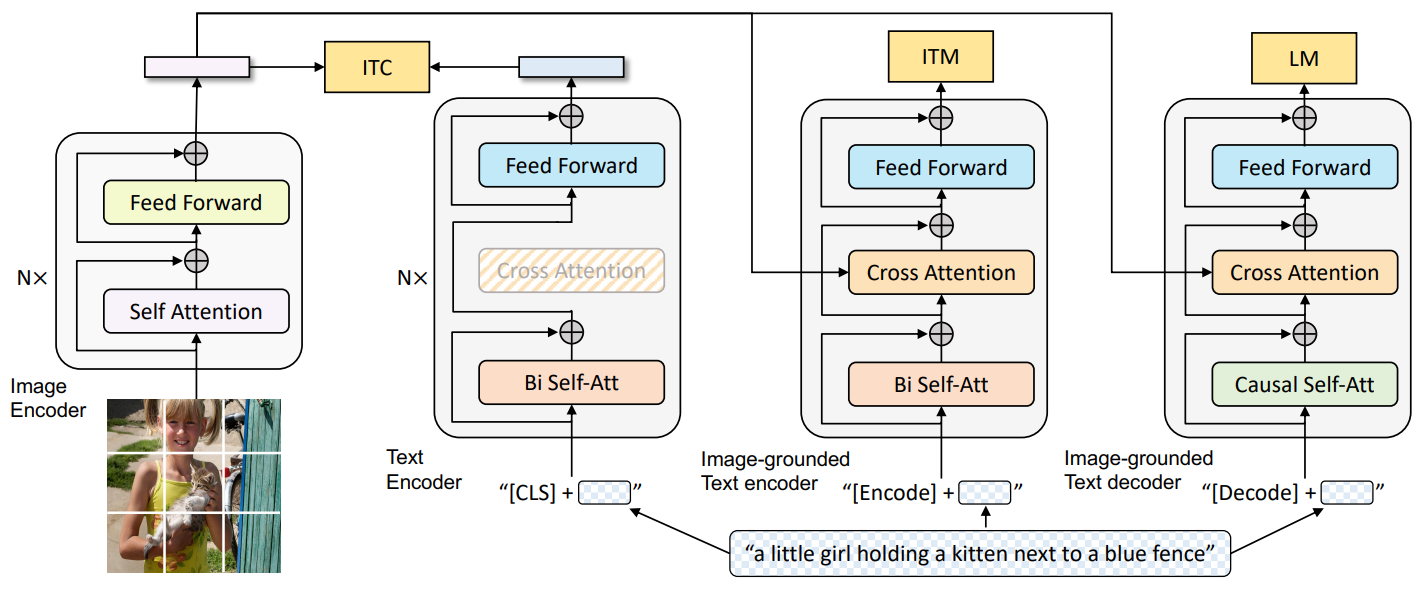
\includegraphics[width=\linewidth]{blip_pretraining.png}
    \caption{BLIP pre-training model architecture: multimodal mixture
of encoder-decoder.}
    \label{fig:blip_pretraining}
\end{figure*}

(1) Unimodal encoders are trained with an image-text contrastive (ITC) loss to align the image and text representations. The image encoder is a visual transformer \cite{dosovitskiy2020image}, which divides an input image into patches and encodes them as a sequence of embeddings. The text encoder is the same as BERT \cite{devlin2018bert}, where a \texttt{[CLS]} token is appended to the beginning of the text input to summarize it.

(2) Image-grounded text encoder is trained with a image-text matching (ITM) loss to distinguish between positive and negative image-text pairs. It has a cross-attention layer between the self-attention layer and the feed forward layer for each transformer block. The output embedding of the \texttt{[Encode]} token is used as the multimodal representation of the image-text pair.

(3) Image-grounded text decoder is trained with a language modeling (LM) loss to generate captions for given images. It replaces the bi-directional self-attention layers in the text encoder with causal self-attention layers. A \texttt{[Decode]} token is used to as the beginning of a sequence.

In order to perform efficient pre-training and improve multi-task learning, the text encoder and text decoder share all parameters except for the self-attention layers. This is enough to capture differences between encoding and decoding tasks.

\subsection{Dataset Bootstraping}

As human-annotated image-text pairs are scarce, vision-language pre-training relies on large-scale image-text pairs automatically collected from the web. However, the texts often do not accurately describe the visual content of the image, making them a noisy supervision. 

To address this, BLIP adds two modules, a captioner and a filter. The learning framework can be seen in Figure \ref{fig:blip_framework}. Both the captioner and the filter are initialized from the same pre-trained MED model, and finetuned individually on the COCO \cite{lin2014microsoft} dataset.

\begin{figure*}
    \centering
    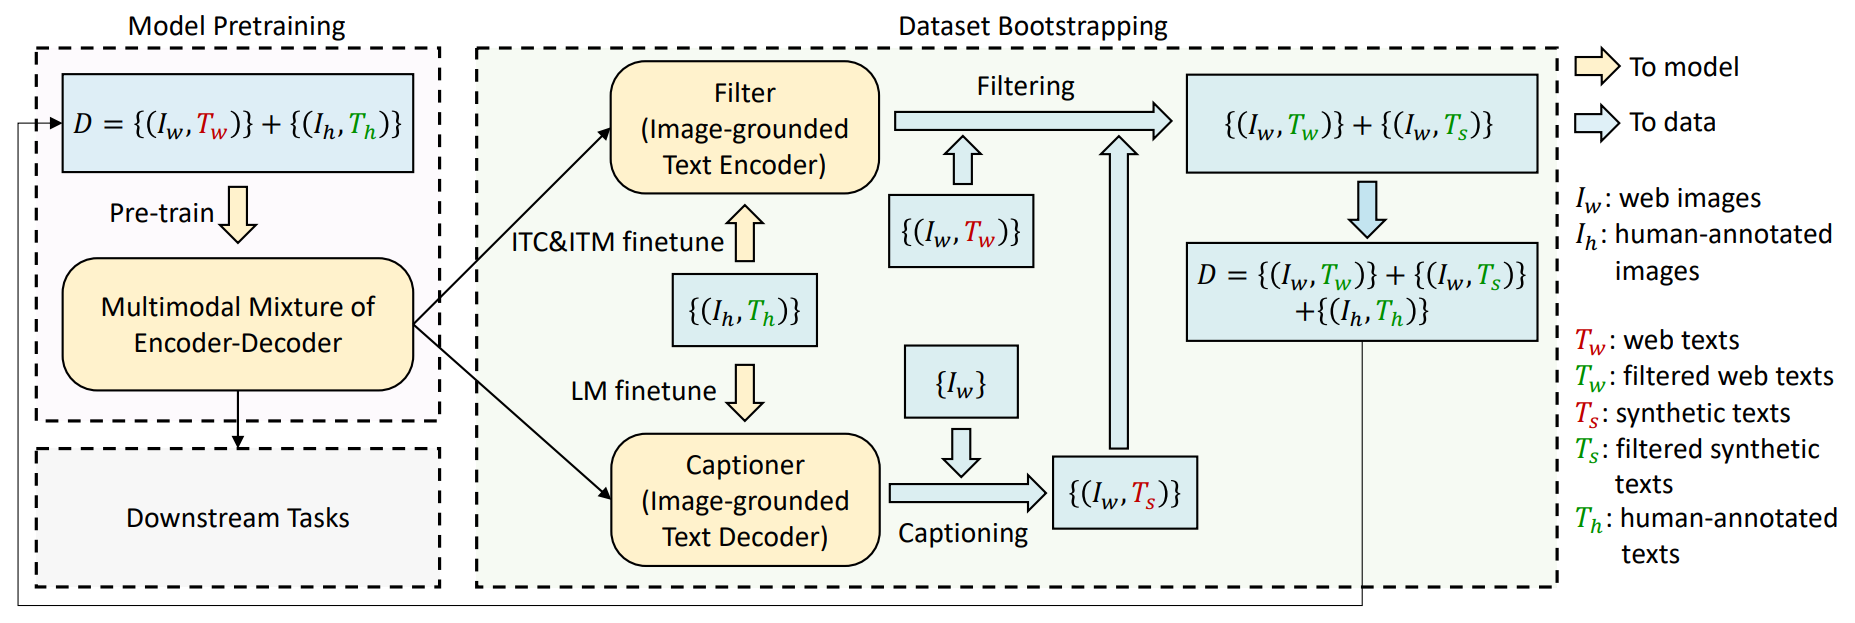
\includegraphics[width=\linewidth]{blip_framework.png}
    \caption{BLIP learning framework: a captioner to produce synthetic captions and a filter to remove noisy captions.}
    \label{fig:blip_framework}
\end{figure*}

The captioner is an image-grounded text decoder. Given the web images, it to generates synthetic captions as additional training samples. The filter is an image-grounded text encoder. It removes noisy captions which do not match their corresponding images. Filtered image-text pairs are combined with the human-annotated pairs to form a new dataset, which is used to pre-train a new model.

\subsection{Finetuning}

On each downstream task, different paths of the pre-trained model are finetuned to achieve different objectives. As the task of our dataset is visual question answering, we will mainly focus on that task.

VQA \cite{antol2015vqa} is a popular vision and language task. Given an image and a question about the image, the task is to provide an accurate answer. VQA\footnote{\url{https://visualqa.org}} dataset is commonly used as a benchmark to evaluate VQA systems. Questions are generally open-ended but multiple choices are provided for some questions. Visual Genome \cite{krishna2017visual} is another popular image-text dataset that was used to finetune the model.

The finetuning architecture for VQA can be seen in Figure \ref{fig:vqa_example}. Image Encoder, Image-grounded Question Encoder and Answer Decoder are used for this task.

\begin{figure*}
    \centering
    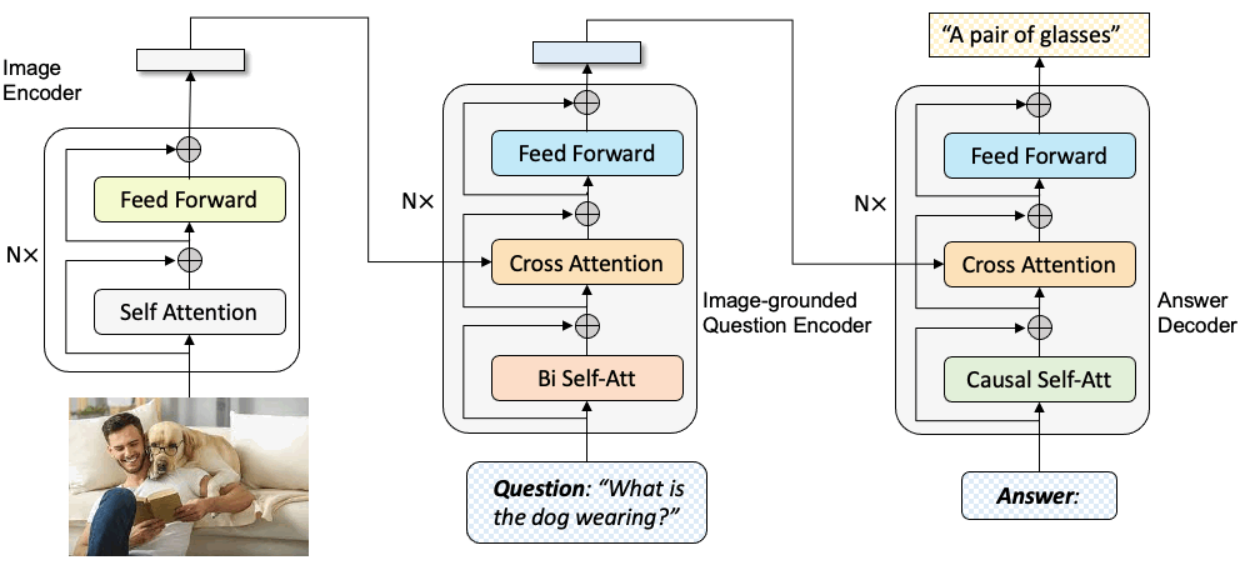
\includegraphics[width=\linewidth]{vqa_example.png}
    \caption{BLIP VQA finetuning architecture.}
    \label{fig:vqa_example}
\end{figure*}

If we compare it to image captioning, VQA requires a more detailed understanding of the image and more complex reasoning \cite{antol2015vqa}. The finetuning architecture for image captioning can be seen in Figure \ref{fig:vqa_example}. The architecture is simpler, only the Image Encoder and Image-grounded Text Decoder are needed.

\begin{figure}
    \centering
    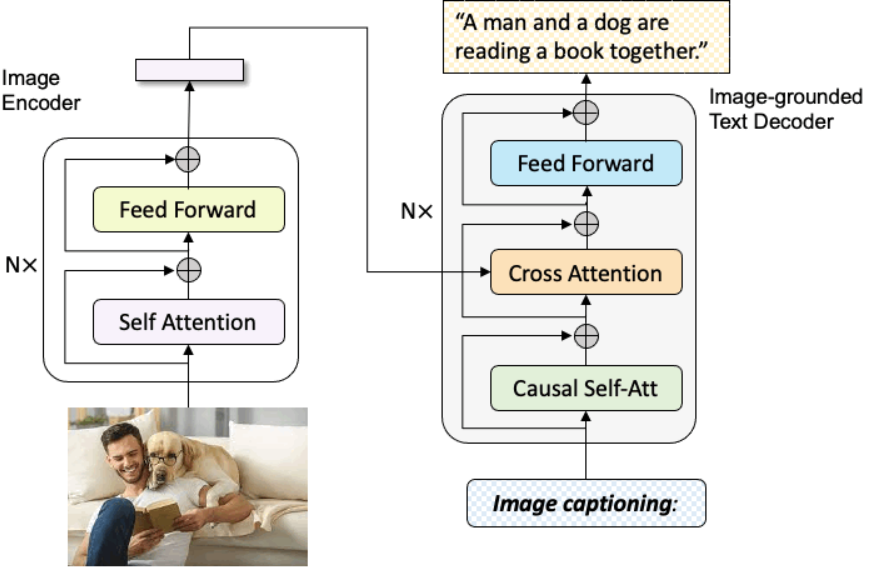
\includegraphics[width=\linewidth]{captioning_example.png}
    \caption{BLIP image captioning finetuning architecture.}
    \label{fig:captioning_example}
\end{figure}

\section{Data}

Three types of questions from Egunean Behin game were selected: figures, cubes and maze. There are multiple questions for each image. Questions require counting figures, colors, cubes and understanding the dimensions of the pictures.

All the images and questions were generated automatically in two steps. First, we generate as many images as we want. Then, we generate multiple questions for each image.

\subsection{Figures}

Images have geometric figures of different types and colors. Figures are selected randomly to create many different images. Images are saved to with a name that contains all the necessary data to create questions. The first two digits correspond to dimension of the image. The next digits correspond to the figures in each position of the image. For example, the name of the image in Figure \ref{fig:figures_example} is figures\_6\_4\_417148\_466526\_041585\_724774.png.

\begin{figure}
    \centering
    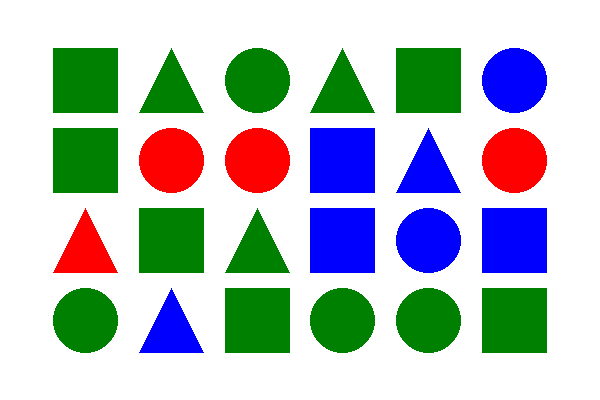
\includegraphics[width=\linewidth]{figures_6_4_417148_466526_041585_724774.png}
    \caption{Figures image example.}
    \label{fig:figures_example}
\end{figure}

18 questions of different types are created for each image. 3 questions about figure, column and row count. 3 questions about figure shape. 3 questions about figure color. 9 questions about figure shape and color combined. Table \ref{tab:figures_example} shows example questions and answers for Figure \ref{fig:figures_example}.

\begin{table}
\centering
\begin{tabular}{llll}
\toprule
Question                  & C       & W1     & W2     \\ \midrule
How many figures?         & 24      & 29     & 26     \\
How many colums?          & 6       & 4      & 8      \\
How many rows?            & 4       & 3      & 2      \\ \midrule
How many triangles?       & 6       & 5      & 8      \\
How many squares?         & 9       & 7      & 11     \\
How many circles?         & 9       & 11     & 8      \\ \midrule
How many red figures?     & 4       & 5      & 3      \\
How many green figures?   & 13      & 15     & 17     \\
How many blue figures?    & 7       & 9      & 10     \\ \midrule
How many red triangles?   & 1       & 3      & 0      \\ 
How many green triangles? & 3       & 4      & 1      \\
How many blue triangles?  & 2       & 4      & 1      \\
How many red squares?     & 0       & 1      & 2      \\
How many green squares?   & 6       & 4      & 5      \\
How many blue squares?    & 3       & 5      & 4      \\
How many red circles?     & 3       & 5      & 4      \\
How many green circles?   & 4       & 3      & 6      \\
How many blue circles?    & 2       & 0      & 3      \\ \bottomrule
\end{tabular}
\caption{Figures questions that correspond with the example image.}
\label{tab:figures_example}
\end{table}

\subsection{Cubes}

See Figure \ref{fig:cubes_example}.

\begin{figure}
    \centering
    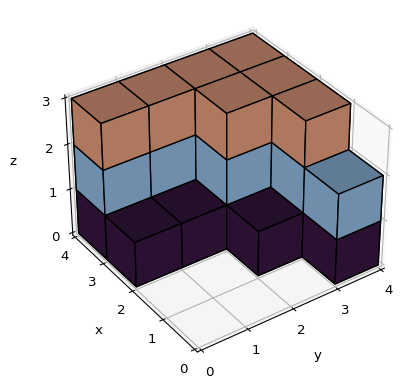
\includegraphics[width=\linewidth]{cubes_4_4_3_0002_0013_1133_3333.png}
    \caption{Cubes image example.}
    \label{fig:cubes_example}
\end{figure}

Many questions of different types are created for each image. The number of questions depends on the dimenssions of the image. 3 questions about total, visible and non visible cubes. 4 questions about number of cubes in each x layer. 4 questions about number of cubes in each y layer. 3 questions about number of cubes in each z layer. Table \ref{tab:cubes_example} shows example questions and answers for Figure \ref{fig:cubes_example}.

\begin{table}
\centering
\begin{tabular}{llll}
\toprule
Question                     & C       & W1     & W2     \\ \midrule
How many cubes in total?     & 26      & 22     & 21     \\
How many visible cubes?      & 17      & 16     & 11     \\
How many non visible cubes?  & 9       & 13     & 10     \\ \midrule
How many cubes in layer x 1? & 2       & 0      & 1      \\
How many cubes in layer x 2? & 4       & 3      & 6      \\
How many cubes in layer x 3? & 8       & 11     & 10     \\
How many cubes in layer x 4? & 12      & 15     & 13     \\ \midrule
How many cubes in layer y 1? & 4       & 6      & 7      \\
How many cubes in layer y 2? & 4       & 3      & 1      \\
How many cubes in layer y 3? & 7       & 9      & 8      \\
How many cubes in layer y 4? & 11      & 8      & 13     \\ \midrule
How many cubes in layer z 1? & 11      & 10     & 12     \\
How many cubes in layer z 2? & 8       & 4      & 11     \\
How many cubes in layer z 3? & 7       & 11     & 10     \\ \bottomrule
\end{tabular}
\caption{Cubes questions that correspond with the example image.}
\label{tab:cubes_example}
\end{table}

\subsection{Maze}

See Figure \ref{fig:maze_example}.

\begin{figure}
    \centering
    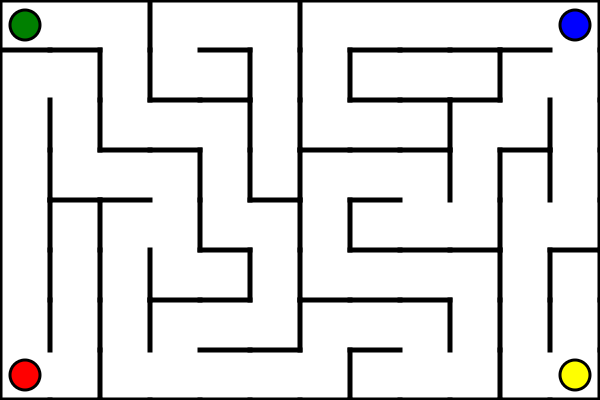
\includegraphics[width=\linewidth]{maze_0_12_8_0_2.png}
    \caption{Maze image example.}
    \label{fig:maze_example}
\end{figure}

\section{Results}

\section{Conclusions}

\bibliography{egunean_behin_vqa}
\bibliographystyle{acl_natbib}

\end{document}
